\section{Présentation de notre interface utilisateur}
\begin{figure}[hbt!]
    \centering
    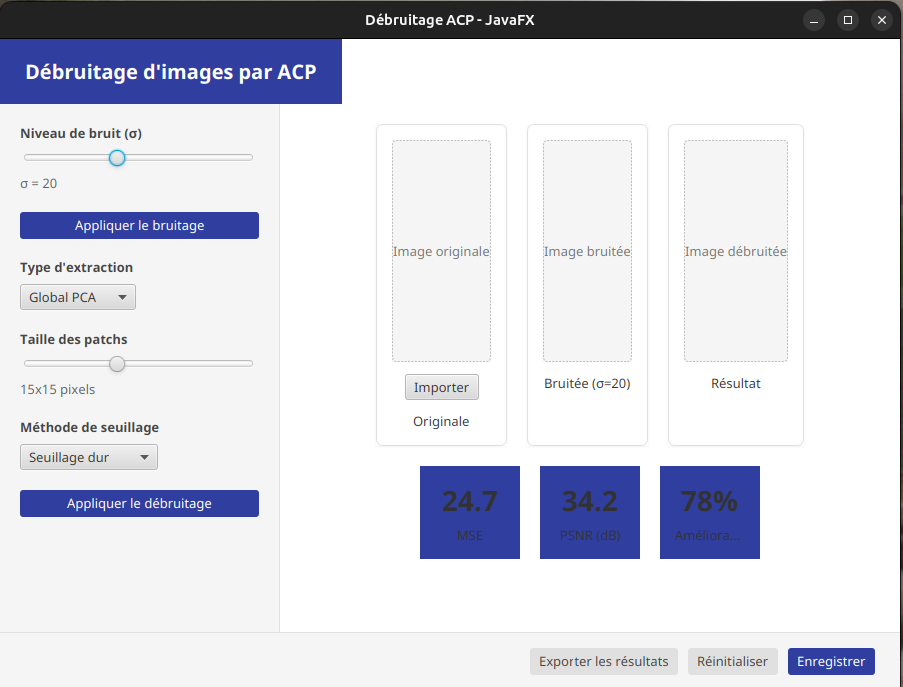
\includegraphics[trim=0cm 0cm 0.5cm 1.5cm, clip, width=0.9\textwidth]{reference/picture/maquette.png}
    \caption{IHM de l'application}
\end{figure}
\subsection{Présentation de l'interface}
L'objectif de l'interface est de proposer les fonctionnalités de notre programme au travers d'une interface graphique permettant de sélectionner les différentes méthodes de seuillage, le type de seuil, la taille des patchs ainsi que la valeur du bruit. \par
Une autre fonctionnalité que nous voulions implémenter est l'affichage de l'image de départ, bruitée ainsi que le résultat final. Il est également important d'afficher les indicateurs de performances associés à la procédure que nous venons d'appliquer sur l'image. \par
Enfin, une action de débruitage optimale est implémentée dans l'IHM afin que les utilisateurs puissent, à partir d'une image bruitée, avoir le meilleur retour des huit méthodes.
\subsection{Justification}
Pour le principe de l'IHM, nous avons voulu suivre les étapes suivantes :
\begin{enumerate}
    \item Charger une image localement
    \item Lui appliquer un bruitage en fonction d'une constante \(\sigma\) choisis par l’utilisateur
    \item Choisir le type d'extraction, la taille des patchs, la méthode de seuillage et le type de seuil
    \item Lecture des indicateurs de performances
    \item Exporter les résultats
\end{enumerate}

Pour le choix du sigma ainsi que la taille des patchs, nous avons choisis des sliders permettant de sélectionner facilement une valeur dans un intervalle. Pour le reste des paramètres, nous avons utilisé des menus déroulants car le choix des possibilités était restreint. \par
Pour les actions de bruitage, débruitage sous paramètres et débruitage optimal, nous avons inséré trois boutons correspondant à chacune de ces actions. \par
Enfin, nous avons la possibilité d'enregistrer, de réinitialiser l'image au travers de deux boutons situés en bas de page